% Propósito: mostrar por qué el enmascarante se presenta al oído no evaluado
% cuando una señal de prueba podría producir una respuesta cruzada.
% Origen: sección \ref{sec:u10-enmascaramiento-aplicado}; esquema funcional
% cualitativo, sin niveles, incrementos ni criterio clínico.
% Descripción accesible: la señal de prueba llega por una ruta directa al oído
% evaluado y por una ruta cruzada discontinua al oído no evaluado. Un
% enmascarante controlado llega al oído no evaluado y reduce allí la
% detectabilidad de la señal cruzada. La respuesta observada no identifica por
% sí sola qué oído detectó la señal.
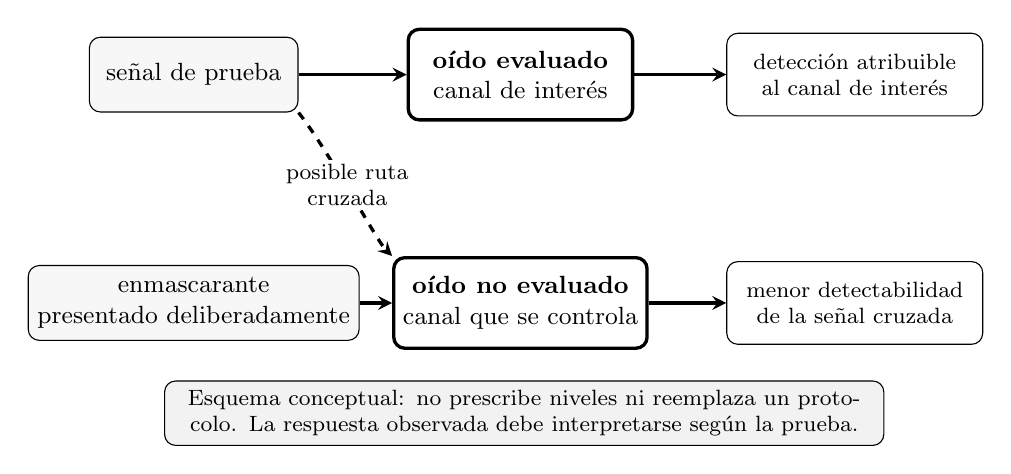
\begin{tikzpicture}[
    x=0.965cm,
    y=1cm,
    >=stealth,
    font=\small,
    senal/.style={
        draw,
        rounded corners,
        minimum width=2.65cm,
        minimum height=0.95cm,
        align=center,
        fill=black!3
    },
    oido/.style={
        draw,
        very thick,
        rounded corners,
        minimum width=2.85cm,
        minimum height=1.15cm,
        align=center
    },
    resultado/.style={
        draw,
        rounded corners,
        minimum width=3.25cm,
        minimum height=1.05cm,
        align=center,
        font=\footnotesize
    }
]
    \node[senal] (prueba) at (1.70,4.25)
        {señal de prueba};
    \node[senal] (masker) at (1.70,1.35)
        {enmascarante\\presentado deliberadamente};

    \node[oido] (evaluado) at (6.00,4.25)
        {\textbf{oído evaluado}\\
         canal de interés};
    \node[oido] (no-evaluado) at (6.00,1.35)
        {\textbf{oído no evaluado}\\
         canal que se controla};

    \node[resultado] (deteccion) at (10.40,4.25)
        {detección atribuible\\
         al canal de interés};
    \node[resultado] (cruzada) at (10.40,1.35)
        {menor detectabilidad\\
         de la señal cruzada};

    \draw[->,very thick] (prueba) -- (evaluado);
    \draw[->,very thick] (evaluado) -- (deteccion);

    \draw[->,very thick,dashed]
        (prueba.south east)
        .. controls (3.50,3.25) and (4.10,2.15) ..
        (no-evaluado.north west);
    \node[
        fill=white,
        inner sep=1.5pt,
        align=center,
        font=\footnotesize
    ] at (3.72,2.85)
        {posible ruta\\cruzada};

    \draw[->,very thick] (masker) -- (no-evaluado);
    \draw[->,very thick] (no-evaluado) -- (cruzada);

    \node[
        draw,
        rounded corners,
        fill=black!5,
        align=center,
        font=\footnotesize,
        text width=8.9cm
    ] at (6.05,-0.05)
        {Esquema conceptual: no prescribe niveles ni reemplaza un protocolo.
         La respuesta observada debe interpretarse según la prueba.};
\end{tikzpicture}
